\documentclass[a4paper, 11pt]{article}

\usepackage[slovene]{babel}
\usepackage[utf8]{inputenc}
\usepackage[T1]{fontenc}
\usepackage{lmodern}
\usepackage{amsmath}
\usepackage{amsfonts}
\usepackage{amssymb}
\usepackage{enumitem}
\usepackage{epsdice}
\usepackage{array}
\usepackage[table]{xcolor}
\usepackage{makecell}
\usepackage{hyperref}
\usepackage{xcolor}
\usepackage{bm}

\usepackage[caption=false]{subfig}

\usepackage{geometry}
\geometry{
 a4paper,
 total={170mm,257mm},
 left=25mm,
 top=25mm,
 }

\newcolumntype{P}[1]{>{\centering\arraybackslash}p{#1}}

\begin{document}

\title{\textbf{\LARGE{Model napovedi odjema električne energije}} \\ Matematika z računalnikom 2023/24}
\author{Karolina Šavli}
\date{Junij 2024}

\maketitle

% =======================================================================================================================
% =======================================================================================================================


\section{Uvod}

Napovedovanje odjema in proizvodnje električne energije je ključno za zagotavljanje stabilnosti in učinkovitosti elektroenergetskega sistema. 
Pravilno načrtovanje proizvodnje in distribucije električne energije je pomembno, saj zmanjšuje tveganje za 
preobremenitve in izpade elektrike. V projektni nalogi bom analizirala in napovedovala odjem električne 
energije gospodinskih odjemalcev. Skozi celoten projekt sem 
uporabljala programski jezik \href{https://www.python.org/}{Python} ter glavne koncepte teorije časovnih vrst. \\

\noindent Glavni cilj projekta je sestaviti model, ki bo kar se da točno napovedal odjem električne energije 
za celotni naslenji dan, torej za naslednjih $24$ ur.

% =======================================================================================================================

\subsection{Teoretična osnova}

\noindent V projektni nalogi se bomo ukvarjali s časovno vrsto $\{X_t\}_t$, torej nekim zaporedjem podatkov. 
Zaradi lažjega razumevanja vsebine si najprej poglejmo
nekaj pomembnih konceptov v okviru časovnih vrst. \\

\noindent Pomemben postopek pri sestavljanju modelov je transformacija časovne vrste v stacionarno.
Časovna vrsta je stacionarna, če ima podobne statistične značilnosti kot vsaka časovno zamaknjena časovna vrsta. 
Ne smemo torej imeti trenda ali sezonskosti.
Stacionarnost lahko preverimo z različnimi formalnimi testi, kot so na primer Augmented Dickey-Fuller (ADF) test,
Kwiatkowski-Phillips-Schmidt-Shin (KPSS) test in Phillips-Perron test.
Pogosti pristopi, da pridemo do stacionarne časovne vrste so logaritmiranje časovne vrste, diferenciranje,
sezonsko diferenciranje, \dots Pri tem si pogosto pomagamo z obravnavo 
avtokorelacijske funkcije (ACF) in parcialno avtokorelacijske funkcije (PACF). 
Ti funkciji sta pomembni, saj opisujeta korelacijo med podatkovnimi točkami v časovni vrsti in prejšnjimi vrednostmi 
časovne vrste (za različne dolžine zamika). Iz teh funkciji lahko razberemo tudi, če imamo sezonsko komponento.
\cite{Stacionarity_V,Brilej_2021} \\

\noindent Namen naše naloge je najti najbolj optimalen model. Za določitev le-tega bomo uporabili kriterij AIC (ang. \emph{Akaike information criterion}),
ki je ocenjevalec napake napovedi in s tem relativne kakovosti statističnih modelov za dan nabor podatkov.
Model, ki ima manjšo vrednost kriterija AIC, je načeloma boljši. 

\subsubsection{Družina modelov ARMA}

\noindent Ker bomo imeli opravka s časovno vrsto, katere lastnosti se s časom ne spreminjajo, bomo
obravnavali model ARMA (ang. \emph{autoregressive moving average process}), ki velja za enega najbolj znanih modelov 
in je osnova vseh modelov s podobnim imemon, ki jih bom v nadaljevanju navedla. 
ARMA(p,q) je združitev modelov AR(p) (ang. \emph{Autoregressive model}) in MA(q) (ang. \emph{Moving-average model}). 
Del AR vključuje regresijo spremenljivke na njene pretekle vrednosti. 
Del MA pa vključuje modeliranje napake kot linearne kombinacije napake, ki se pojavljajo v preteklosti.
ARMA model je oblike

\begin{equation}
    \label{ARIMA}
    X_t = \mu +  \sum_{i=1}^{p}{\varphi_i X_{t-i}} + \sum_{i=1}^{q}{\theta_i \varepsilon_{t-i}} + \varepsilon_t \,,
\end{equation}

\noindent kjer so $\varphi_1, \dots, \varphi_p$ ter $\theta_1, \dots, \theta_q$ parametri
modela, $\varepsilon_t, \varepsilon_{t-1}, \dots$ pa je beli šum, ki je običajno
normalno porazdeljen. \\

\noindent ARMA predpostavlja stacionarno vrsto. Če vrsta ni popolnoma stacionarna, kar je običajno razvidno 
že kar iz ACF in PACF, uporabimo posplošitev modela ARMA, to je model ARIMA(p,d,q) (ang. \emph{autoregressive integrated moving average}).
Na kratko, ARIMA vrednosti podatkov nadomesti z diferenciranimi vrednostmi reda d, saj na tak način dobi stacionarne podatke.
V primeru, da imamo sezonsko komponento, uporabimo model SARIMA (sezonska ARIMA). Parametre v modelu
SARIMA(p,d,q)(P,D,Q)[S] lahko razdelimo na nesezonske (p,d,q) in sezonske (P,D,Q,S). 
p pove koliko korakov nazaj bomo gledali (preberemo iz grafa PACF), 
d določi kolikokrat smo diferencirali,
q pa pove število zgodovinskih napak, ki vplivajo na trenutno vrednost (preberemo iz grafa ACF).
Sezonski P predstavlja red sezonskega AR(P), 
D pove kolikokrat smo sezonsko diferencirali,
Q določa red sezonskega MA(Q), 
S pa je perioda. \cite{SARIMA_param} \\

\noindent Model SARIMA(p,d,q)(P,D,Q)[S] je odlike

\begin{equation}
    \label{SARIMA}
    X_t = \mu + \sum_{i=1}^{p}{\varphi_i X_{t-i}} + \sum_{i=1}^{q}{\theta_i \varepsilon_{t-i}} + \color{blue} \sum_{i=1}^{P}{\phi_i X_{t-S}} + \sum_{i=1}^{Q}{\Theta_i \varepsilon_{t-S}}  \color{black} +  \varepsilon_t\,,
\end{equation}

\noindent kjer so $\phi_1, \dots, \phi_P$ in $\Theta_1, \dots, \Theta_Q$ dodatni parametri modela. Opazimo, da 
smo Formuli~\eqref{ARIMA} dodali moder del iz Formule~\eqref{SARIMA}, da smo dobili SARIMA model. \\

\noindent Model lahko še dodatno nadgradimo, in sicer z vključitvijo eksogenih spremenljivk, torej nekih zunanjih podatkov. Tako
dobimo model SARIMAX(p,d,q)(P,D,Q)[S], ki je oblike

\begin{equation}
    \label{SARIMAX}
    X_t = \mu + \sum_{i=1}^{p}{\varphi_i X_{t-i}} + \sum_{i=1}^{q}{\theta_i \varepsilon_{t-i}} + \color{blue} \sum_{i=1}^{P}{\phi_i X_{t-S}} + \sum_{i=1}^{Q}{\Theta_i \varepsilon_{t-S}}  \color{red}  + \sum_{r=1}^{R}{\beta_i Y_{i_{t}}} \color{black} +  \varepsilon_t\,,
\end{equation}

\noindent kjer je ob času $t$, $Y_{i_t}$ $i$-ta eksogena spremenljvika s koeficientom $\beta_i$. \cite{ARMA_ARIMA_SARIMA_SARIMAX}

\subsubsection{Model GARCH}

V modelih družine ARMA je privzeta konstantna varianca. Ni pa nujno, da je le-ta vedno konstantna, zato
vpeljimo še model GARCH, ki se običajno uporablja ravno na podatkih, ki nimajo konstantne variance. 
Model GARCH($p_G$,$q_G$) je definiran kot

\begin{equation}
    \label{GARCH}
    \sigma^2_t = \omega + \sum_{i=1}^{p_G}{\alpha_i \varepsilon_{t-i}^2} + \sum_{i=1}^{q_G}{\beta_i \sigma_{t-i}^2} \,,
\end{equation}

\noindent kjer so $\alpha_1, \dots, \alpha_{p_G}$ in $\beta_1, \dots, \beta_{q_G}$ koeficienti, ki 
jih poskušamo določiti. $\sigma^2_t$ je pogojna varianca ob času $t$, $\varepsilon_t$ pa predstavlja beli šum
ob času $t$. \cite{ArimaGarch}

\subsubsection{Model SARIMAX-GARCH}

\noindent Da v modelu iz družine ARMA, npr. modelu SARIMAX, opišemo tudi varianco, ki ni konstantna, in s tem dobimo bolj
točen model, lahko 
konstruiramo model SARIMAX-GARCH. Da dobimo model združimo Formuli~\eqref{SARIMAX} in ~\eqref{GARCH} ter dobimo

\begin{equation}
    \label{SARIMAX_GARCH}
    X_t = \mu + \sum_{i=1}^{p}{\varphi_i X_{t-i}} + \sum_{i=1}^{q}{\theta_i \varepsilon_{t-i}} + \sum_{i=1}^{P}{\phi_i X_{t-S}} + \sum_{i=1}^{Q}{\Theta_i \varepsilon_{t-S}}  + \sum_{r=1}^{R}{\beta_i Y_{i_{t}}} \color{orange} + \sqrt{\sigma_t} z_t \color{black} \,,
\end{equation}

\noindent kjer je $z_t \sim \text{NEP}(0,1)$. \cite{ArimaGarch}



% =======================================================================================================================
% =======================================================================================================================

\pagebreak

\section{Osnovna analiza časovne vrste}

\noindent Podjetje \href{https://gen-i.si/}{GEN-I} je v obliki excel razpredelnice pripravilo tabelo podatkov, sestavljeno iz $7$ stolpcev:
\begin{itemize}
    \item  \texttt{DateTimeStartUTC}: univerzalni koordinirani čas,
    \item  \texttt{DateTimeStartCET}: srednjeevropski čas,
    \item  \texttt{Odjem ACT}: odjem električne energije gospodinjskih odjemalcev (tistih brez sončne elektrarne),
    \item  \texttt{Temperatura ACT}: dejanska temperatura, 
    \item  \texttt{Temperatura FC}: s strani GEN-I napovedana temperatura,
    \item  \texttt{Sevanje ACT}: dejansko sevanje in
    \item  \texttt{Sevanje FC}: s strani GEN-I napovedano sevanje. 
\end{itemize}

\begin{figure}[h!]
    \centering
    \caption{Tabela podatkov, 2021-2024}\par\medskip
    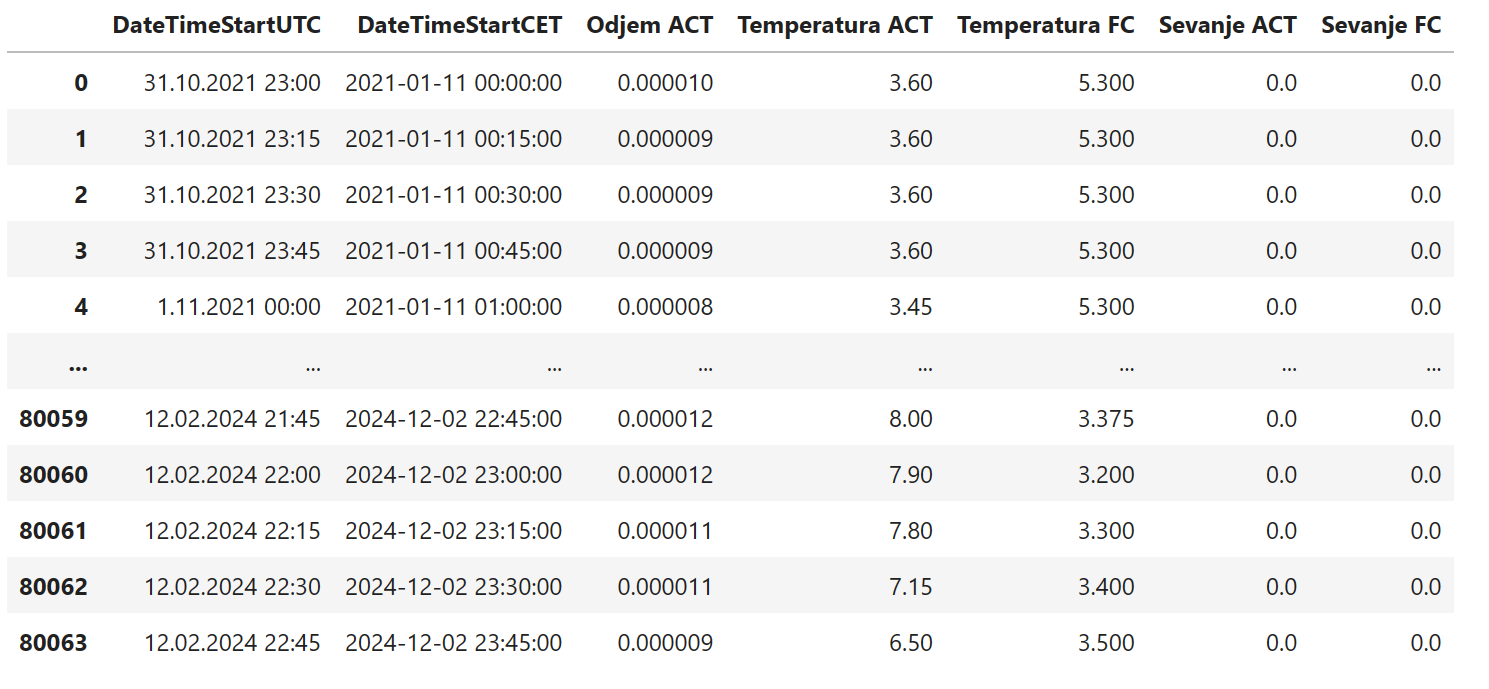
\includegraphics[width=0.9\textwidth]{tabela.png}
\end{figure}

\noindent V analizi sem uporabljala vse stolpce, razen stolpca \texttt{DateTimeStartUTC}, saj je v 
okviru časa bolj relavanten stolpec \texttt{DateTimeStartCET}. Podatki v stolpcu \texttt{Odjem ACT} so bili
s strani GEN-I normalizirani in zaradi boljše preglednosti in v izogib morebitnemu zaokroževanju 
ugrajenih funkcij, sem jih pomnožila z  $10^6$. \\
Podatki so podani za obdobje od $1.~\text{novembra}~2021$ do $29.~\text{februarja}~2024$,
na vsakih $15$ minut. Tako ima tabela ima vsega skupaj $81696$ vrstic.

% =======================================================================================================================

\subsection{Odjem električne energije}

\noindent Slika~\ref{fig:odjem_EE} prikazuje odjem električne energije za obdobje od 
$1.~\text{novembra}~2021$ do $29.~\text{februarja}~2024$. 
Opazna je sezonskost - odjem je znatno večji jeseni in pozimi, zaradi povečane uporabe energije za ogrevanje in 
razsvetljevo, saj se število ur dnevne svetlobe podaljša. \\

\begin{figure}[h!]
    \centering
    \caption{Odjem električne energije, 2021-2024}\par\medskip
    \label{fig:odjem_EE}
    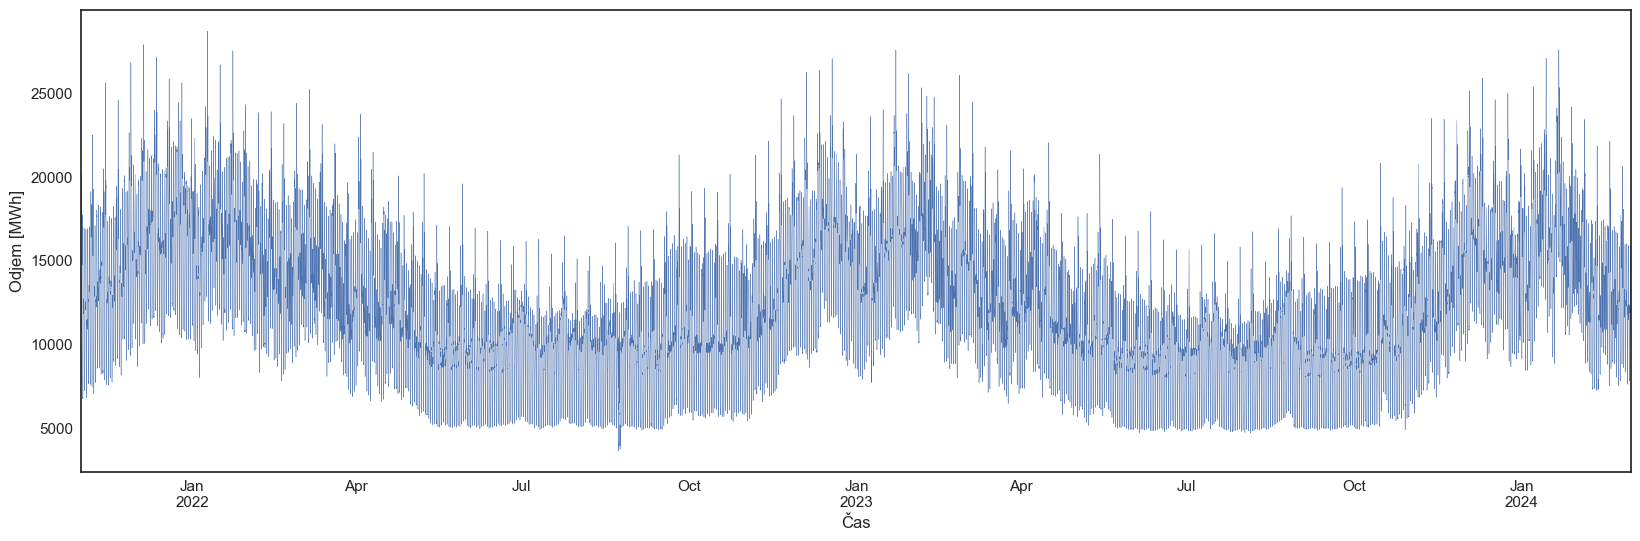
\includegraphics[width=0.9\textwidth]{odjem_EE.png}
\end{figure}

\noindent S Tabele~\ref{Tab:opisne_statistike} preberemo, da je povprečna poraba električne energije gospodinjskih odjemalcev
okrog $12240{,}53 $, minimalna dosežena vrednost je $3629{,}32$, maksimalna pa $28736{,}80$. Vrednosti varirajo
za okrog $4167{,}98$. \\

\begin{table}[!h]
    \centering
    \caption{Opisne statistike porabe električne energije, 2021-2024}\par\medskip
    \label{Tab:opisne_statistike}
    \begin{tabular}{c||c|c|c|c|c}
              & Min & Max & Povprečje & Mediana & Standardni odklon \\ \hline \hline
        Odjem & $3629{,}32$ & $28736{,}80$ & $12240{,}53$ & $11708{,}50$ & $4167{,}98$ \\ 
    \end{tabular}
\end{table}

\noindent Odjem električne energije si poglejmo še na ravni tedna. Opazimo, da 
je od ponedeljka do petka odjem najmanjši ponoči in se veča vse do viška okrog 18 ure, nato pa hitro pade. 
V soboto in nedeljo pa je prvi višek porabe dopoldne, drugi pa ponovno okrog 18 ure, kar je opazno s Slike~\ref{fig:odjem_teden}, 
ki prikazuje odjem 
električne energije v drugem tednu septembra 2023. 
Imamo torej sezonskost na dnevni ravni.

\begin{figure}[h!]
    \centering
    \caption{Odjem električne energije po urah, drugi teden septembra 2023}\par\medskip
    \label{fig:odjem_teden}
    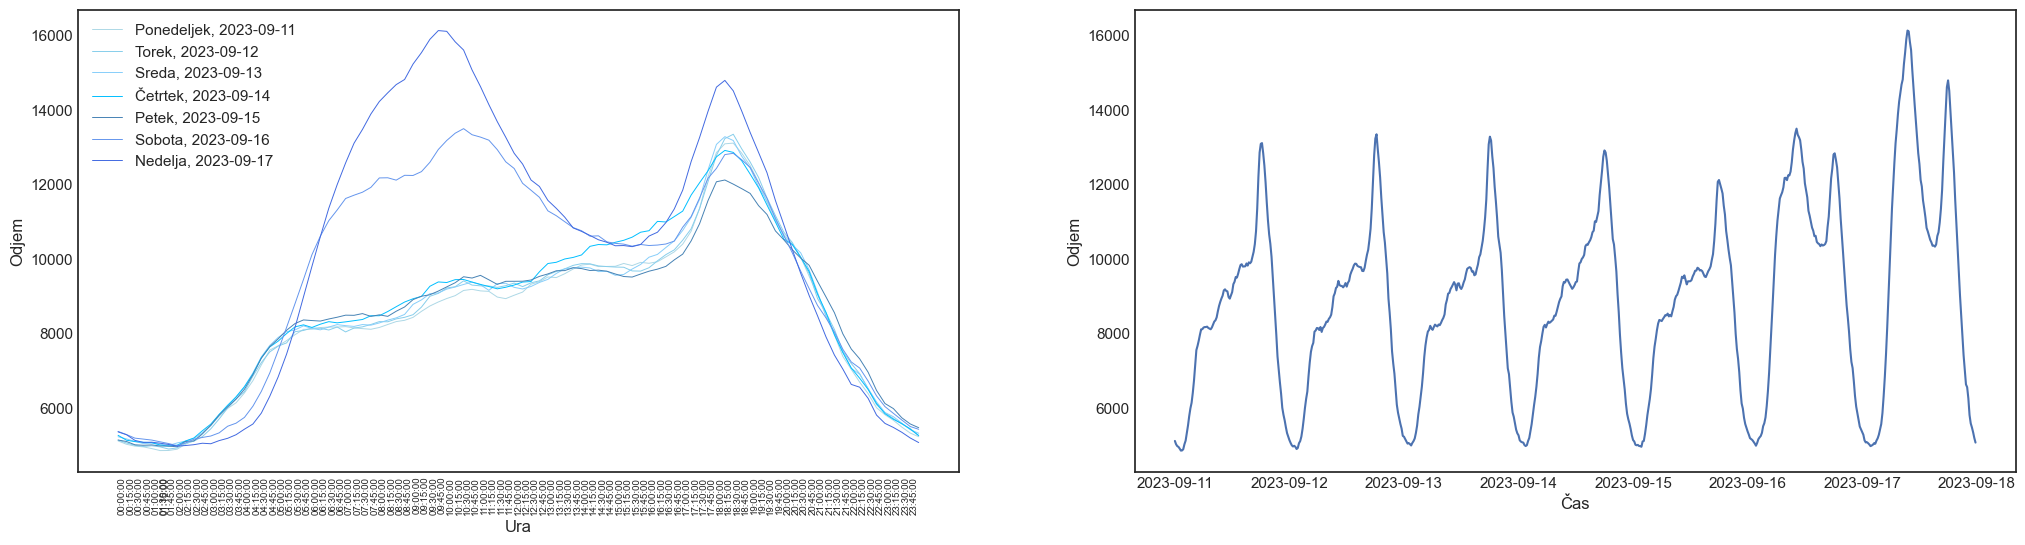
\includegraphics[width=0.9\textwidth]{odjem_teden.png}
\end{figure}

\noindent Zaključimo lahko, da je naša časovna vrsta visokofrekvenčna, ima sezonsko komponentno ter njeno povprečje ni konstantno.

% =======================================================================================================================

\subsection{Povezava med odjemom in temperaturo ter sevanjem}

\noindent Smislno se zdi, da obstaja povezava med odjemom električne energije ter
temperaturo in sevanjem. S pomočjo Slike~\ref{fig:temp_sevanje} ugotovimo, da
nižja temperatura pomeni višji odjem in obratno. 
Povezave med sevanjem in odjemom pa ni opaziti; sklepam da zato, ker 
ne analiziramo samooskrbnih odjemalcev (tistih, ki imajo svojo sončno elektrarno). 

\begin{figure}[h!]
    \centering
    \caption{Povezava med odjemom in temperaturo ter sevanjem, 2021-2024}\par\medskip
    \label{fig:temp_sevanje}
    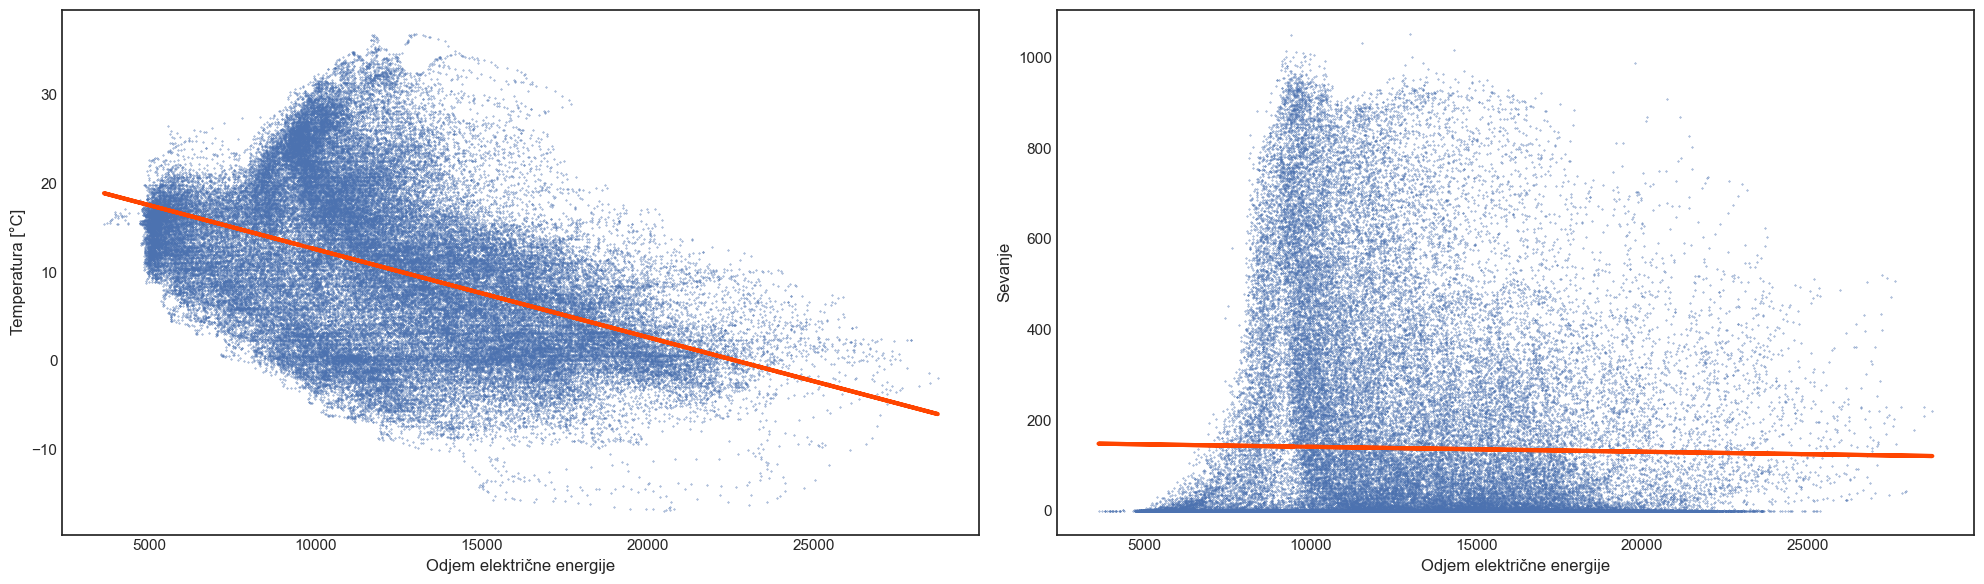
\includegraphics[width=0.9\textwidth]{temp_sevanje.png}
\end{figure}

\noindent V nadaljevanju bomo v upanju boljše napovedi v naše modele kot 
eksogeni spremenljivki vključili tudi temperaturo in sevanje. 


% =======================================================================================================================
% =======================================================================================================================


\section{Napredna analiza in izbira modela}

\subsection{Izbira družine modelov}

Časovna vrsta odjema je visofrekvenčna, ima sezonsko komponento in njeno povprečje ni konstantno.
Odločimo se, da bomo s pomočjo teorije časovnih vrst konstruirali model iz družine ARMA. 
Razmislek o izbiri modela začnemo z ARIMO. Ker pa imamo v podatkih očitno sezonskost, lahko ARIMO nadgradimo v SARIMO, 
ki dodatno
upošteva še sezonske vzorce. Ker bi radi vključili tudi eksogeni spremenljivki (temperatura in sevanje), model
dodatno nadgradimo v model SARIMAX.
Vemo pa tudi, da ima ta družina modelov težavo predvsem pri napovedih časovnih vrst, ki se jim  
skozi čas spreminja varianca. Da bo naše napovedovanje bolj učinkovito, bomo model SARIMAX povezali z modelom GARCH, 
ki se uporablja ravno za modeliranje volativnih podatkov.~\cite{ArimaGarch} Konstruirati torej želimo model
SARIMAX-GARCH, ki smo ga opisali s Formulo~\eqref{SARIMAX_GARCH}.


% =======================================================================================================================

\subsection{Odstranitev sezonskosti in pridobitev stacionarnosti}

Da bomo lahko indentificiralni potencialne modele iz družine ARMA, moramo najprej 
originalno časovno vrsto (Slika~\ref{fig:odjem_EE})
narediti stacionarno. \\

\noindent Ker so naši podatki volatilni najprej naredimo \textbf{logaritmične donose} 
(ang. \emph{log returns}). Če z $W_t$ označimo originalno časovno vrsto odjema električne energije, so logaritmični donosi
definirani kot časovna vrsta $ Y_t = \ln \left( \frac{W_t}{W_{t-1}} \right) $. Slednja časovna vrsta je prikazana na
Slika~\ref{fig:log_returns}.

\begin{figure}[h!]
    \centering
    \caption{Logaritmični donosi odjema električne energije, 2021-2024}\par\medskip
    \label{fig:log_returns}
    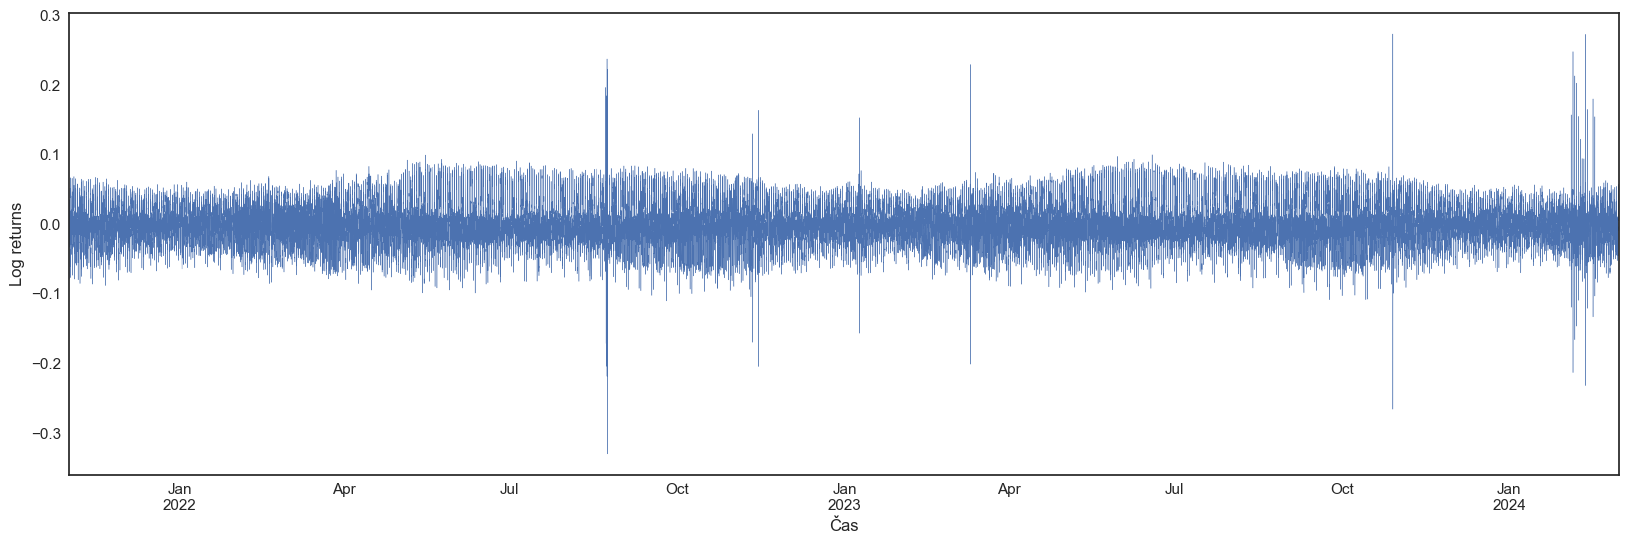
\includegraphics[width=0.9\textwidth]{log_returns.png}
\end{figure}

\begin{figure}[h!]
    \centering
    \caption{Vzorčna avtokorelacijska in parcialna avtokorelacija funkcija časovne vrste logaritmičnih donosov}\par\medskip
    \label{fig:log_returns_acf_pacf}
    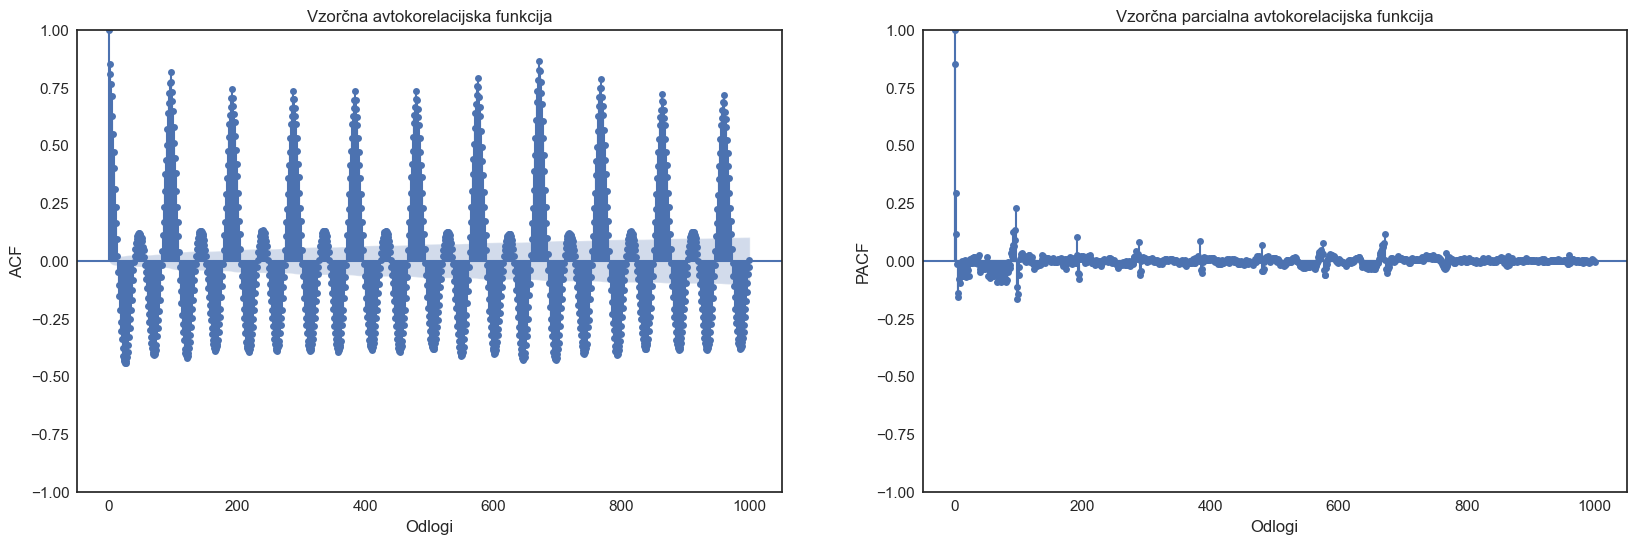
\includegraphics[width=0.9\textwidth]{log_returns_acf_pacf.png}
\end{figure}

\noindent Slika~\ref{fig:log_returns_acf_pacf} prikazuje 
ACF in PACF logaritmičnih donosov do odloga $1000$ (to je
malo manj kot dva tedna). Z grafov je očitno, da časovna vrsta ni stacionarna. Opazna je sezonska komponentna, in sicer $96$, 
kar je ravno en dan \footnote{Podatki so podani na $15$ minut in $15\,\text{min} \cdot 96 = 1440\,\text{min}$, kar je ravno en dan.}. \\

\noindent Da dosežemo stacionarnost, se je potrebno sezonskosti znebiti, zato bomo podatke naprej \textbf{sezonsko diferencirali}.
Nova časovna vrsta bo $Z_t = Y_t - Y_{t-96} = \bigtriangledown_{96}Y_t$. Prikazana je na Sliki~\ref{fig:ts_diff}, njeni ACF in PACF pa na Sliki~\ref{fig:ts_diff_acf_pacf}.

\begin{figure}[h!]
    \centering
    \caption{Časovna vrsta $Z_t$, 2021-2024}\par\medskip
    \label{fig:ts_diff}
    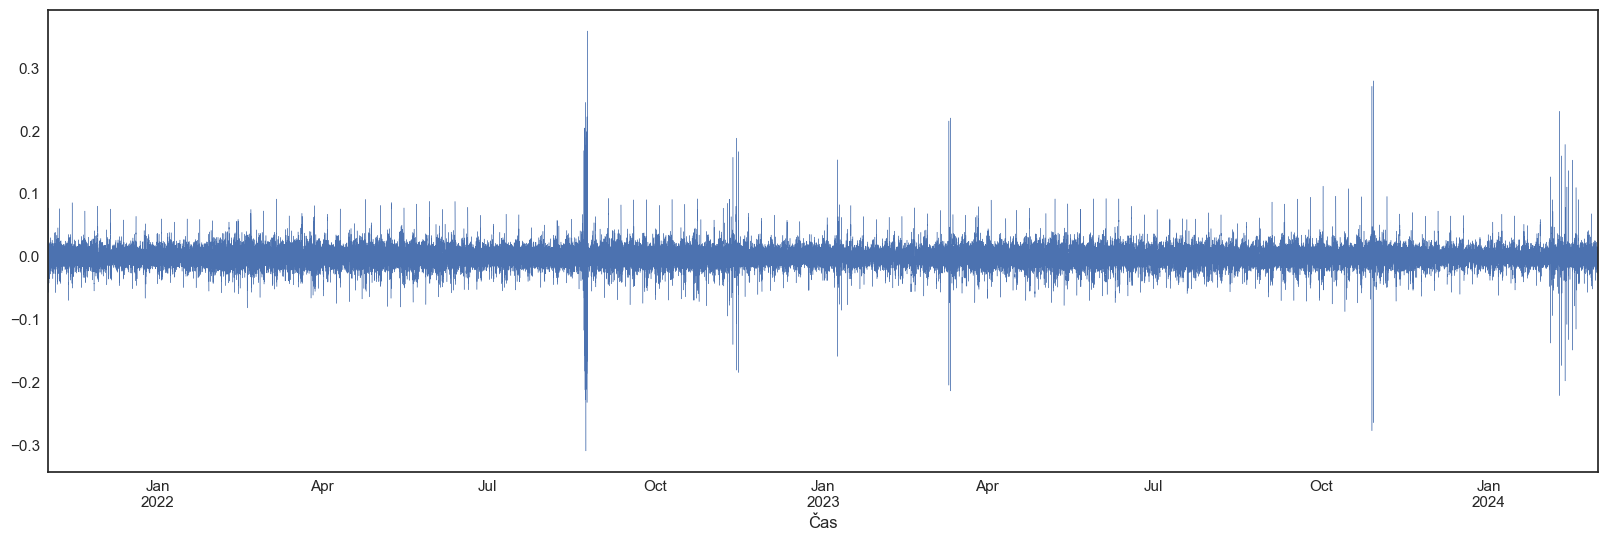
\includegraphics[width=0.9\textwidth]{ts_diff.png}
\end{figure}

\begin{figure}[h!]
    \centering
    \caption{Vzorčna avtokorelacijska in parcialna avtokorelacija funkcija časovne vrste $Z_t$}\par\medskip
    \label{fig:ts_diff_acf_pacf}
    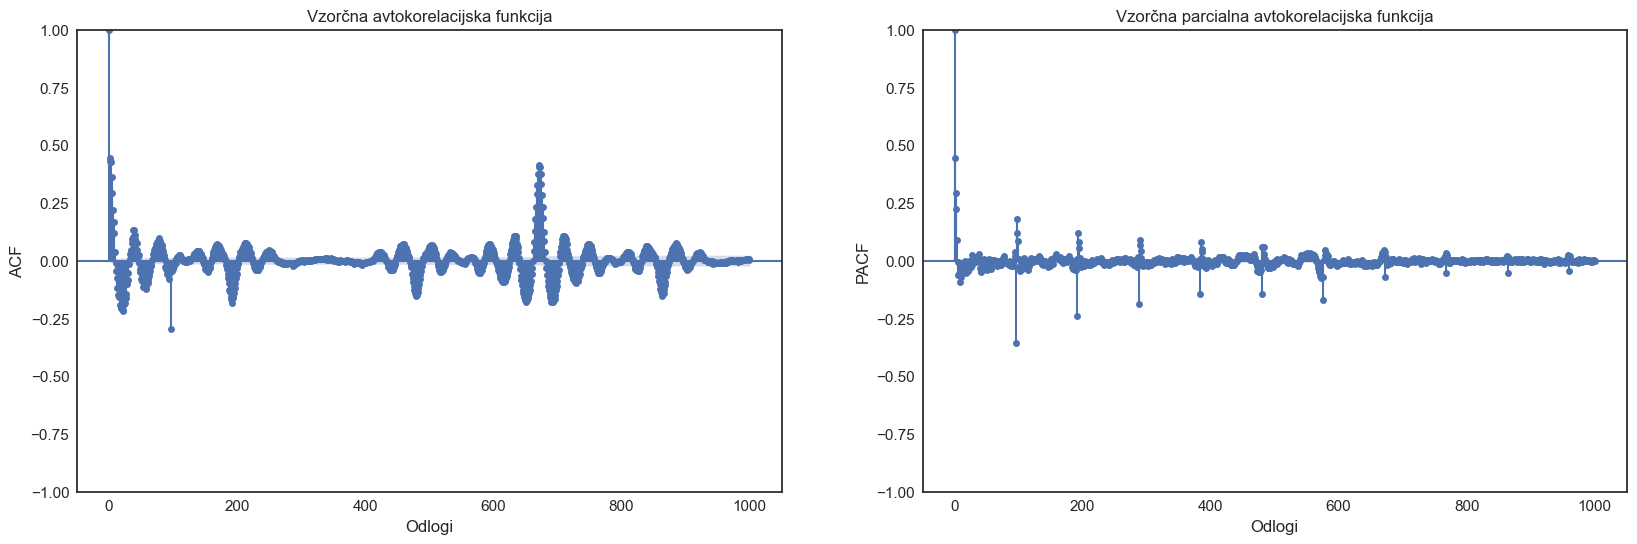
\includegraphics[width=0.9\textwidth]{ts_diff_acf_pacf.png}
\end{figure}

\noindent Na grafu ACF opazimo ponavljanje vzorca, kar pomeni, da časovna vrsta $Z_t$ še kar ni stacionarna. 
Še enkrat jo diferenciramo, tokrat \textbf{ne}sezonsko. Dobimo časovno vrsto $X_t = Z_t - Z_{t-1} = \bigtriangledown{Z_t}$. 
Prikazana je na Sliki~\ref{fig:ts_diff_2}, njeni ACF in PACF pa na Sliki~\ref{fig:ts_diff_2_acf_pacf}.

\begin{figure}[h!]
    \centering
    \caption{Časovna vrsta $X_t$, 2021-2024}\par\medskip
    \label{fig:ts_diff_2}
    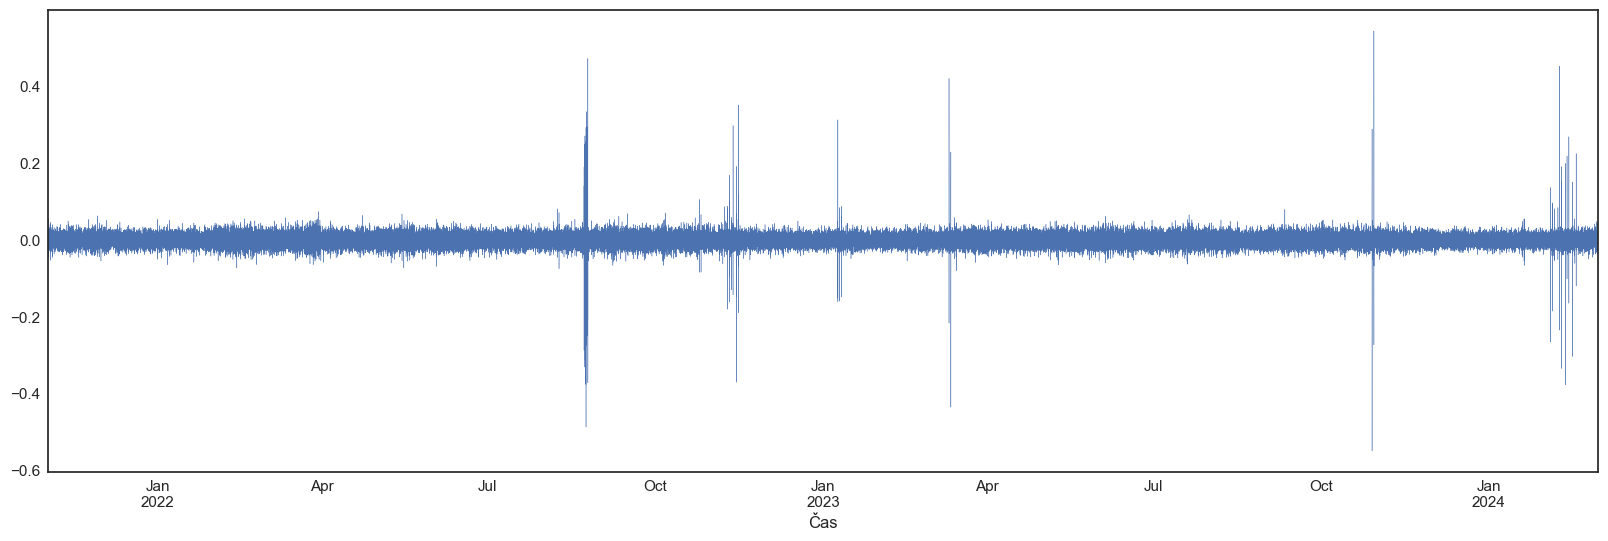
\includegraphics[width=0.9\textwidth]{ts_diff_2.png}
\end{figure}

\begin{figure}[h!]
    \centering
    \caption{Vzorčna avtokorelacijska in parcialna avtokorelacija funkcija časovne vrste $X_t$}\par\medskip
    \label{fig:ts_diff_2_acf_pacf}
    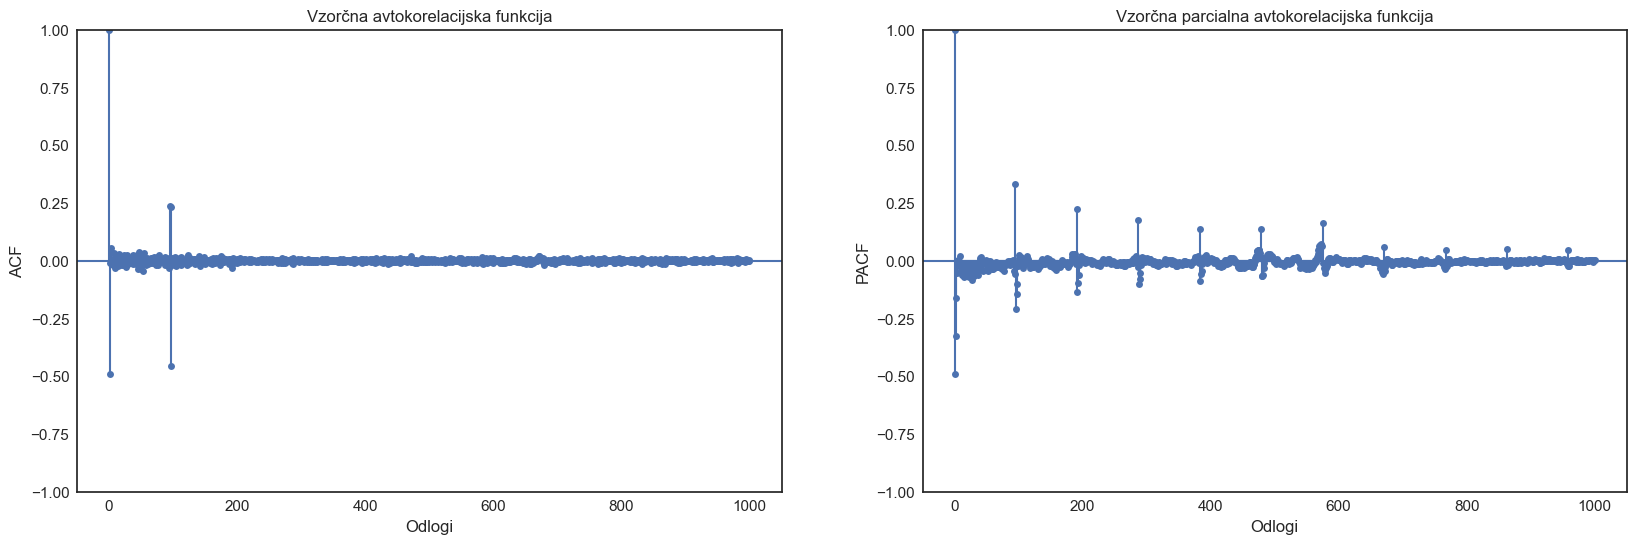
\includegraphics[width=0.9\textwidth]{ts_diff_2_acf_pacf.png}
\end{figure}

\begin{figure}[h!]
    \caption{Vzorčna avtokorelacijska in parcialna avtokorelacija funkcija časovne vrste $X_t$, odlogi do 100}\par\medskip
    \centering
    \label{fig:ts_diff_2_acf_pacf_do_100}
    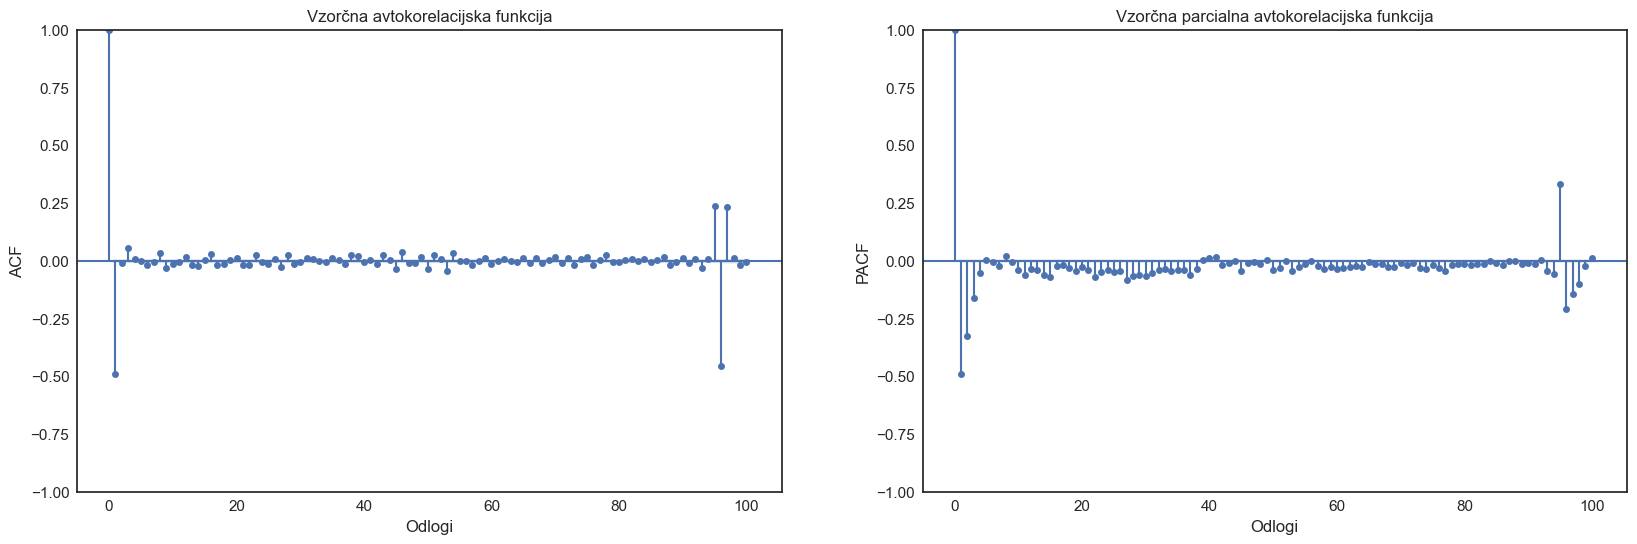
\includegraphics[width=0.9\textwidth]{ts_diff_2_acf_pacf_do_100.png}
\end{figure}

\noindent Dobljena časovna vrsta $X_t$ na podlagi ACF in PACF (Slika~\ref{fig:ts_diff_2_acf_pacf}) 
zgleda stacionarno in tudi formalni testi ADF, 
KPSS in Phillips-Perron potrdijo njeno stacionarnost. 
Časovna vrsta je torej primerna za izbero parametrov modela SARIMAX. 

% =======================================================================================================================

\subsection{Identifikacija modela SARIMAX}

\noindent Na podlagi ACF in PACF (Slika~\ref{fig:ts_diff_2_acf_pacf}) stacionarne časovne vrste $X_t$, izberimo parametre 
modela SARIMAX(p,d,q)(P,D,Q)[S], ki je podan z Enačbo~\eqref{SARIMAX}. \\

\noindent Ker smo časovno vrsto enkrat sezonsko diferencirali bo $\text{D} = 1$ in ker smo jo enkrat 
navadno diferencirali bo $\text{d} = 1$. Perioda je enaka $96$, torej je $\text{S} = 96$. \\

\noindent Za določitev sezonskih parametrov P in Q gledamo korelacije pri odlogih, ki so večkratniki periode S. Pri
PACF visoko korelacijo opazimo predvsem pri $96$ in $192$, nato pa se z vsako dodatno periodo manjša. Parameter P je torej 
$1$ ali več; predlagala bi $1$, $2$ ali $3$. 
Pri ACF pa je občutna korelacija zgolj pri $96$, zato izberemo $\text{Q} = 1$. \\

\noindent Za lažjo določitev nesezonskih parametrov p in q bomo gledali ACF in PACF do prve periode (torej do odloga 96). 
Slednje je prikazano na Sliki~\ref{fig:ts_diff_2_acf_pacf_do_100}. Tako iz PACF, kot tudi iz ACF, je opazna večja korelacija
pri prvih nekaj urah in v uri tik pred periodo. V modelu bomo zato zagotovo vključili prvih nekaj $15$-minutnih intervalov, 
saj le-ti kažejo močan vpliv. \\


\noindent Izbrala sem nekaj potencialnih modelov SARIMAX, kjer sem kot eksogeni spremenljivki podala temperaturo in sevanje.
Modele sem trenirala na $75~\%$ podatkov, to je od $1.~\text{novembra}~2021$ do $4.~\text{avgusta}~2023$. Na preostanku podatkov 
pa sem izvajala teste napovedi. 
Vrednosti kriterija AIC za posamezne modele so prikazane v Tabeli~\ref{Tab:SARIMA_AIC}. 
Najmanjšo vrednostjo kriterija AIC ima model SARIMAX(4,1,5)(0,1,0)[96] \footnote{S Tabele~\ref{Tab:SARIMA_AIC} 
je razvidno, da sem za sezonska parametra P in Q v vseh primerih izbrala 
vrednost $0$, čeprav predvidevam, da bi bile bolj optimalne višje vrednosti. Te modele sem poskusila zagnati, 
vendar moj računalnik ni vrnil nobenega rezultata, ker očitno ni dovolj zmogljiv. Predvidevam da bi z 
vključitvijo vrednosti P in Q, prišla do še bolj optimalnih rezultatov.}. 

\begin{table}[!ht]
    \centering
    \caption{Vrednost kriterija AIC za izbrane modele iz družine SARIMAX}\par\medskip
    \label{Tab:SARIMA_AIC}
    \begin{tabular}{c|c}
        Model & AIC \\ \hline
        SARIMAX(1,1,0)(0,1,0)[96] & $-338588{,}046$ \\ 
        SARIMAX(0,1,1)(0,1,0)[96] & $-346718{,}519$ \\ 
        SARIMAX(1,1,1)(0,1,0)[96] & $-346768{,}583$ \\ 
        SARIMAX(2,1,1)(0,1,0)[96] & $-347555{,}507$ \\ 
        SARIMAX(3,1,2)(0,1,0)[96] & $-347573{,}394$ \\ 
        SARIMAX(4,1,3)(0,1,0)[96] & $-278981{,}698$ \\ 
        SARIMAX(5,1,4)(0,1,0)[96] & $-345287{,}413$ \\ 
        SARIMAX(5,1,5)(0,1,0)[96] & $-345310{,}105$ \\ 
        SARIMAX(4,1,5)(0,1,0)[96] & $\mathbf{-347619{,}304}$ \\ 
        SARIMAX(6,1,5)(0,1,0)[96] & $-345325{,}842$ \\ 
        SARIMAX(6,1,6)(0,1,0)[96] & $-345342{,}972$ \\ 
        SARIMAX(5,1,6)(0,1,0)[96] & $-345351{,}794$ \\
    \end{tabular}
\end{table}

\noindent Izbran imamo model SARIMAX, v naslednjem koraku pa na podoben način izberimo še model GARCH, da bomo
prišli do želenega modela SARIMAX-GARCH. 

% =======================================================================================================================

\subsection{Izbira modela SARIMAX-GARCH}

Model GARCH(p, q) bomo konstruirali na rezidualih izbranega modela SARIMAX. Preizkusili bomo $6$ kombinacij 
parametrov p in q, in sicer $(1,1), (1,2), (2,1), (2,2), (1,3)$ ter $(3,1)$. 
Na podlagi vrednosti kriterija AIC se odločimo za model \textbf{SARIMAX(4,1,5)(0,1,0)[96]-GARCH(1,3)}, saj
je iz Tabele~\ref{Tab:GARCH_AIC} razvidno, da ima najmanjšo vrednost kriterija AIC. Ima tudi manjšo vrednost 
AIC kot SARIMAX(4,1,5)(0,1,0)[96]-\textbf{GARCH(0,0)}, kar je enako SARIMAX(4,1,5)(0,1,0)[96]. S povezavo
SARIMAX in GARCH torej res pridemo do boljšega modela. 

\begin{table}[!ht]
    \centering
    \caption{Vrednost kriterija AIC za izbrane modele SARIMAX(4,1,5)(0,1,0)[96]-GARCH(p,q)}\par\medskip
    \label{Tab:GARCH_AIC}
    \begin{tabular}{c|c}
        SARIMAX-GARCH(p,q) & AIC \\ \hline
        $(0,0)$ & $-347619{,}304$ \\ 
        $(1,1)$ & $-365754{,}448$ \\ 
        $(1,2)$ & $-366056{,}218$ \\ 
        $(2,1)$ & $-365434{,}577$ \\ 
        $(2,2)$ & $-365843{,}673$ \\ 
        $(1,3)$ & $\mathbf{-366134{,}335}$ \\ 
        $(3,1)$ & $-365252{,}576$ \\ 
    \end{tabular}
\end{table}


% =======================================================================================================================

\subsection{Izbran model}

Na podlagi vrednosti kriterija AIC smo se odločili za SARIMAX(4,1,5)(0,1,0)[96]-GARCH(1,3). 
Ključni koeficienti izbranega modela v Formuli~\eqref{SARIMAX_GARCH} so:

\begin{itemize}
    \item  AR del: $\varphi_1 = -0{,}3686,\, \varphi_2 = -0{,}4185,\, \varphi_3 = -0{,2894},\, \varphi_4 = 0{,0486}$
    \item  MA del: $\theta_1 = - 0{,}3311,\, \theta_2 = 0{,}1863,\, \theta_3 = 0{,}0931,\, \theta_4 = -0{,}2059,\, \theta_5 = 0{,}0583$
    \item  sezonskih del: parametrov nimamo, ker sta P in Q enaka $0$
    \item  GARCH del: $\alpha_1 = 0{,}2,\, \beta_1 = 0{,}2333,\, \beta_2 = 0{,}2333,\, \beta_3 = 0{,}2333$
    \item  Eksogene spremenljivke: koeficient pri temperaturi je enak $-0{,}0003$, pri sevanju pa $3{,}747 \cdot 10^{-6}$
\end{itemize}

\noindent Sevanje ima torej pri modelu napovedi zelo majhen vpliv, vendar sem preverila in ugotovila da je model z vključitvijo sevanja
še vedno malce boljši. Model je nasploh z vključitvijo eksogenih spremenljivk preverjeno bolj točen. 


% =======================================================================================================================
% =======================================================================================================================

\section{Testiranje izbranega modela SARIMAX-GARCH}

Izbran model SARIMAX-GARCH uporabimo za napovedovanje odjema električne energije za različne dni v testnem obdobju
(od $5.~\text{avgusta}~2023$ do $12.~\text{februarja}~2024$). Izbrala sem si $6$ različnih dni, narisala njihove napovedi ter
jih prikazala na Sliki~\ref{fig:napovedi_vse}.

\begin{figure}[!ht]
    \centering
    \caption{Napovedi odjema električne energije za izbrane datume}\par\medskip
    \label{fig:napovedi_vse}
    \begin{minipage}[c]{0.48\linewidth}
        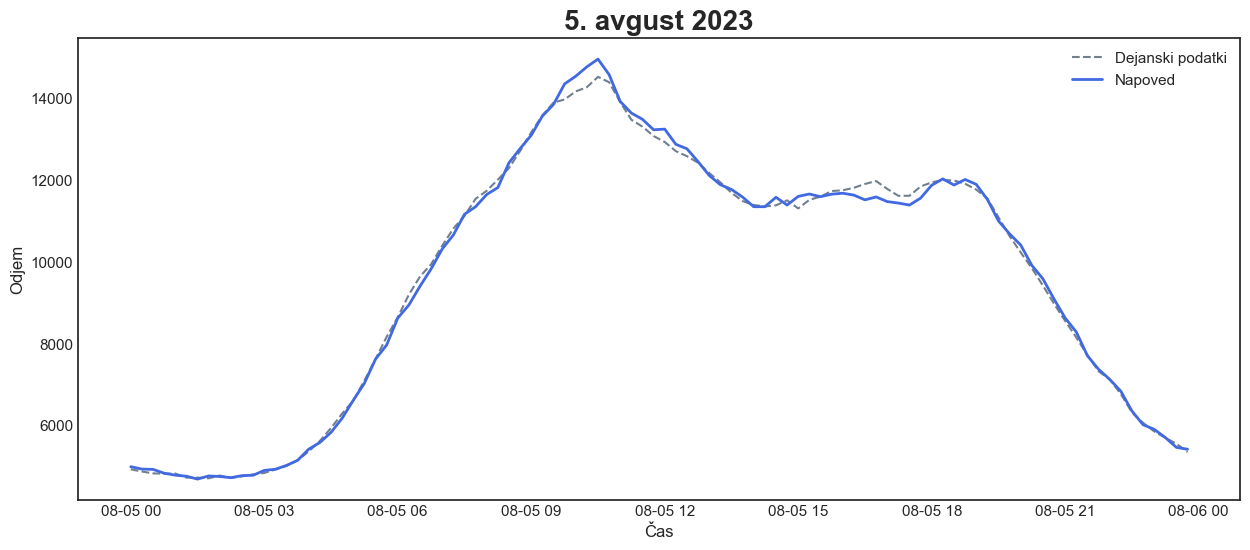
\includegraphics[width=\linewidth]{napoved_1.png}
    \end{minipage}
    \hfill
    \begin{minipage}[c]{0.48\linewidth}
        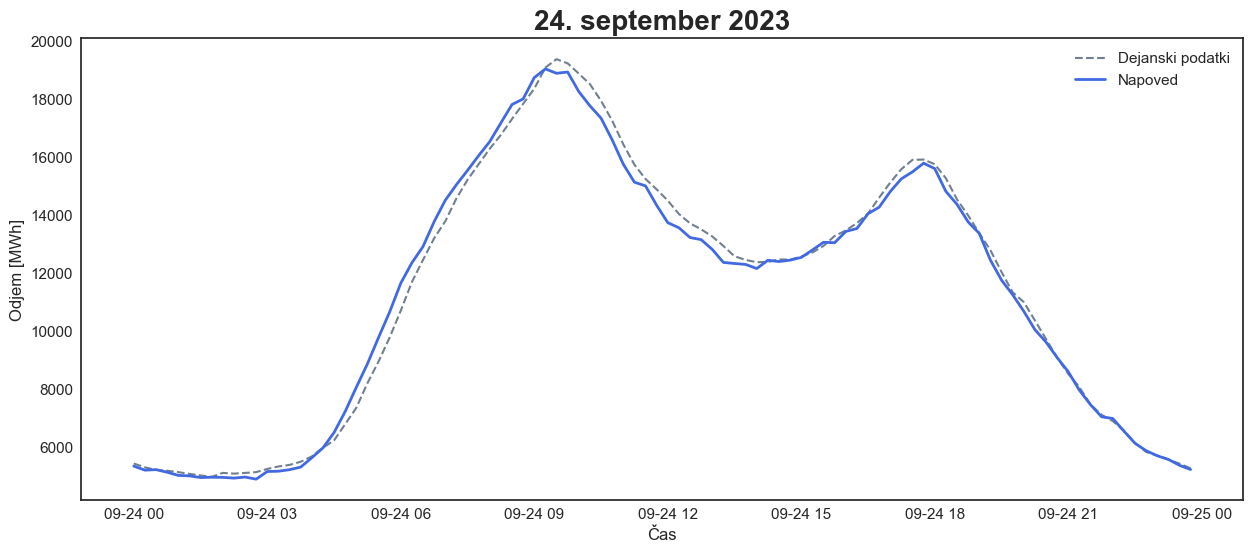
\includegraphics[width=\linewidth]{napoved_2.png}
    \end{minipage}
\end{figure}
\begin{figure}[!ht]
    \centering
    \begin{minipage}[c]{0.48\linewidth}
        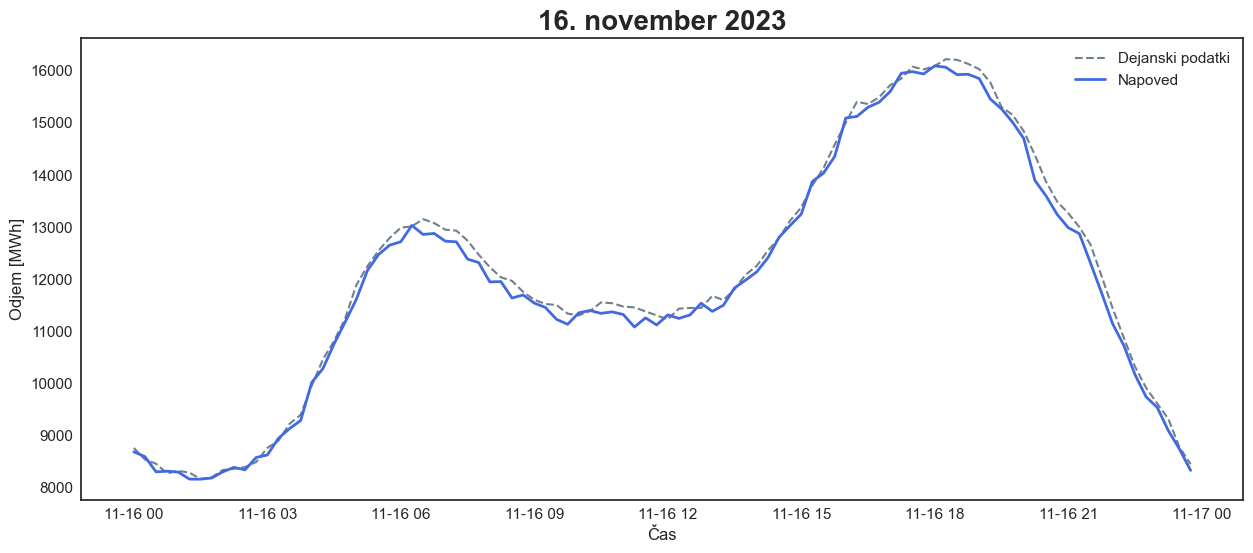
\includegraphics[width=\linewidth]{napoved_3.png}
    \end{minipage}
    \hfill
    \begin{minipage}[c]{0.48\linewidth}
        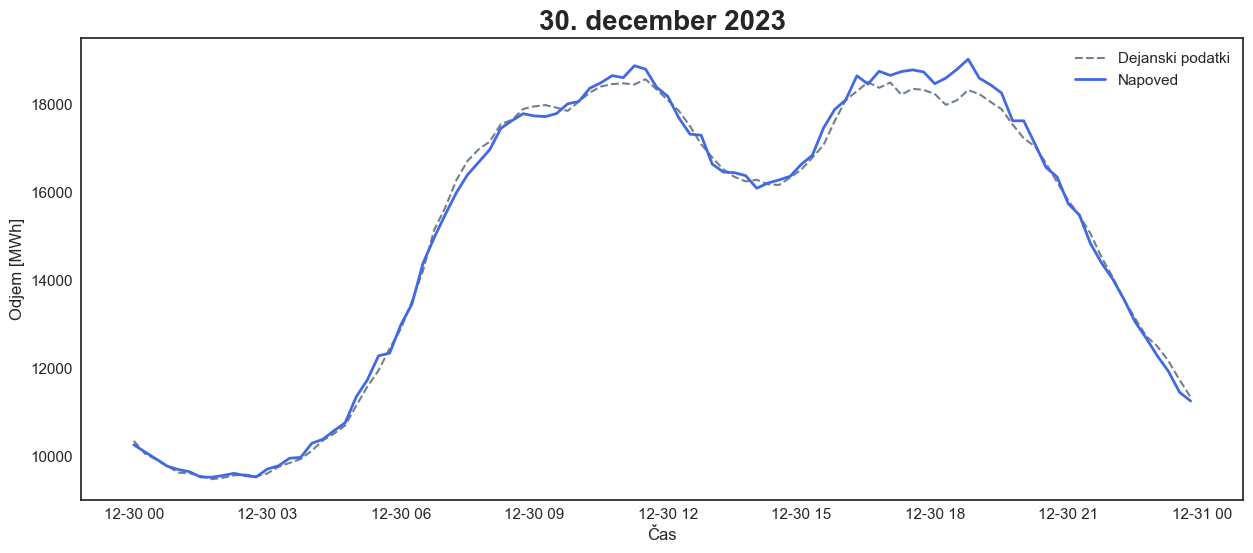
\includegraphics[width=\linewidth]{napoved_4.png}
    \end{minipage}
\end{figure}
\begin{figure}[!ht]
    \centering
    \begin{minipage}[c]{0.48\linewidth}
        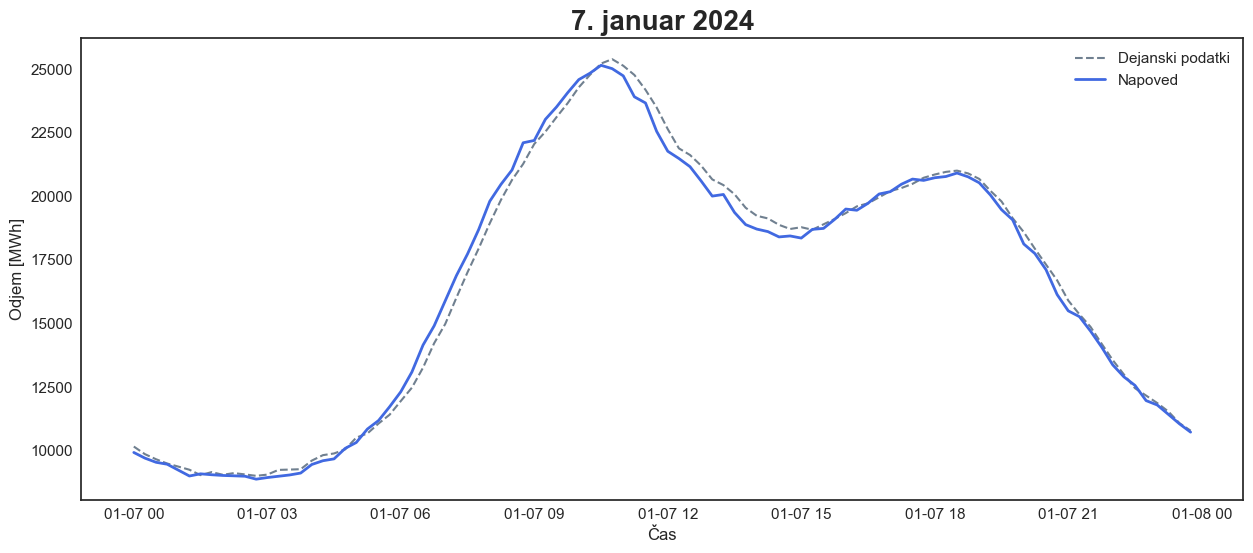
\includegraphics[width=\linewidth]{napoved_5.png}
    \end{minipage}
    \hfill
    \begin{minipage}[c]{0.48\linewidth}
        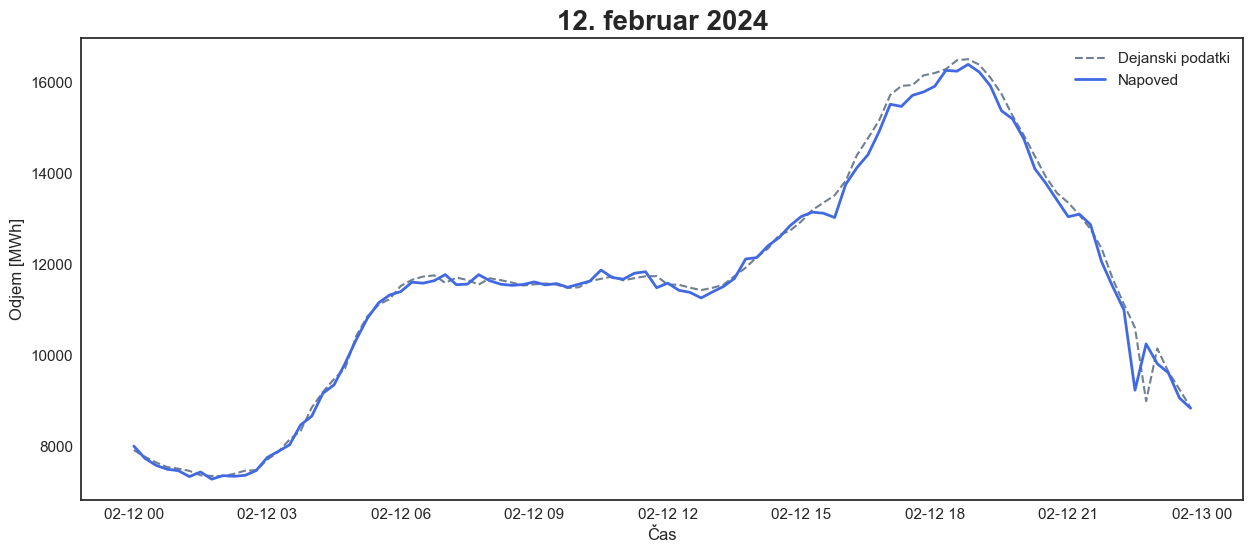
\includegraphics[width=\linewidth]{napoved_6.png}
    \end{minipage}
\end{figure}

\noindent Prileganje napovedi dejanski vrednosti se zdi zelo dobra, vseeno pa si
poglejmo napaki RMSE (ang. \emph{Root-mean-square deviation}) in 
MAPE (ang. \emph{Mean absolute percentage error}), ki ju izračunamo po formulah:

$$
RMSE = \sqrt{\frac{1}{96}\sum_{t=1}^{96}{(W_t-\hat{W_t})^2}} \quad \textrm{in} \quad
MAPE = \frac{1}{96}\sum_{t=1}^{96}{\frac{W_t-\hat{W_t}}{W_t}} \,,
$$

\noindent kjer je $W_t$ dejanska vrednost odjema, $\hat{W_t}$ pa napovedana. \\

\noindent Vrednosti napak RMSE in MAPE za izbrane napovedi so zapisane v Tabeli~\ref{Tab:RMSE_MAPE} in 
v povprečju znašajo RMSE $261{,}926$, MAPE pa $1{,}478~\%$. \\


\begin{table}[!ht]
    \centering
    \caption{Vrednost napake RMSE in MAPE za izbrane datume}\par\medskip
    \label{Tab:RMSE_MAPE}
    \begin{tabular}{l|c|c}
        Datum & RMSE & MAPE \\ \hline
        5. avgust 2023 & 156,600 & 1,104 \\ 
        24. september 2023 & 365,372 & 2,392 \\ 
        16. november 2023 & 176,901 & 1,199 \\ 
        30. december 2023 & 224,123 & 1,046 \\ 
        7. januar 2024 & 399,578 & 1,839 \\ 
        12. februar 2024 & 248,981 & 1,287 \\ \hline
        Povprečje & 261,926 & 1,478 \\ 
    \end{tabular}
\end{table}


\noindent Napaki RMSE in MAPE sem izračunala še posebej za zadnji teden septembra 2023 in 
prvi teden februarja 2024. Rezultati so prikazani v Tabeli~\ref{Tab:RMSE_MAPE_sept}  in v Tabeli~\ref{Tab:RMSE_MAPE_feb}. 
Iz Tabele~\ref{Tab:RMSE_MAPE_sept} zgleda kot, da se večja napaka pojavi za vikend, vendar glede na rezultat iz
Tabele~\ref{Tab:RMSE_MAPE_feb} ne moremo tega z gotovostjo trditi. 


\begin{table}[!ht]
    \centering
    \caption{Vrednost napake RMSE in MAPE zadnji teden septembra 2023}\par\medskip
    \label{Tab:RMSE_MAPE_sept}
    \begin{tabular}{c||c|c|c|c|c|c|c||c}
        ~ & Ponedeljek & Torek & Sreda & Četrtek & Petek & Sobota & Nedelja & Povprečje\\ \hline
        RMSE & $98{,}768$ & $73{,}987$ & $84{,}263$ & $90{,}712$ & $182{,}816$ & $220{,}022$ & $336{,}630$ & $155{,}314$ \\ 
        MAPE & $0{,}813$ & $0{,}707$ & $0{,}800$ & $0{,}773$ & $1{,}442$ & $1{,}679$ & $2{,}406$ & $1{,}231$\\ 
    \end{tabular}
\end{table}


\begin{table}[!ht]
    \centering
    \caption{Vrednost napake RMSE in MAPE prvi teden februarja 2024}\par\medskip
    \label{Tab:RMSE_MAPE_feb}
    \begin{tabular}{c||c|c|c|c|c|c|c||c}
        ~ & Ponedeljek & Torek & Sreda & Četrtek & Petek & Sobota & Nedelja & Povprečje\\ \hline
        RMSE & $136{,}451$ & $129{,}370$ & $418{,}558$ & $324{,}463$ & $168{,}860$ & $353{,}170$ & $420{,}640$ & $278{,}788$\\ 
        MAPE & $0{,}867$ & $0{,}817$ & $2{,}041$ & $1{,}522$ & $1{,}108$ & $1{,}670$ & $2{,}377$ & $1{,}486$\\ 
    \end{tabular}
\end{table} 


% =======================================================================================================================
% =======================================================================================================================

\section{Zaključek}

\noindent S pomočjo transformacije podatkov, preverjanja ACF, PACF ter vrednosti kriterija AIC pridemo do 
modela napovedi odjema električne energije gospodinjskih odjemalcev. 
Kot optimalen model izberemo SARIMAX(4,1,5)(0,1,0)[96]-GARCH(1,3). \\

\noindent Napoved izbranega modela dobro opisuje dejanske vrednosti, kar je lepo razvidno iz grafov napovedi. 
Formalno, povprečna napaka RMSE znaša okrog $260$, 
MAPE pa $1{,}5~\%$. Tekom dela ugotovimo tudi, da vključitev eksogenih podatkov prispeva k bolj točni napovedi. \\

\noindent Če bi modele testirala s pomočjo bolj zmogljivega računalnika, sem prepričana, da bi prišla do vsaj malo boljših
napovedi, saj bi vključila še sezonske parametre. 
Kljub vsemu pa so rezultati napovedi dobri in predvsem smiselni.


% =======================================================================================================================
% =======================================================================================================================

{\small
\bibliographystyle{abbrv}
\bibliography{literatura.bib}}


\end{document}
